\phantomsection
\setstretch{1.5}
\justify
\fontsize{14}{16}\selectfont
\setlength{\parindent}{0pt}
\chapter*{IV. Część Praktyczna } 
\addcontentsline{toc}{chapter}{\textnormal{IV. Część Praktyczna}}
\fontsize{12}{14}\selectfont

\phantomsection
\setstretch{1.5}
\justify
\fontsize{14}{16}\selectfont
\setlength{\parindent}{0pt}
\section*{1. Opis działania programu} 
\addcontentsline{toc}{section}{\textnormal{1. Opis działania programu}}
\fontsize{12}{14}\selectfont


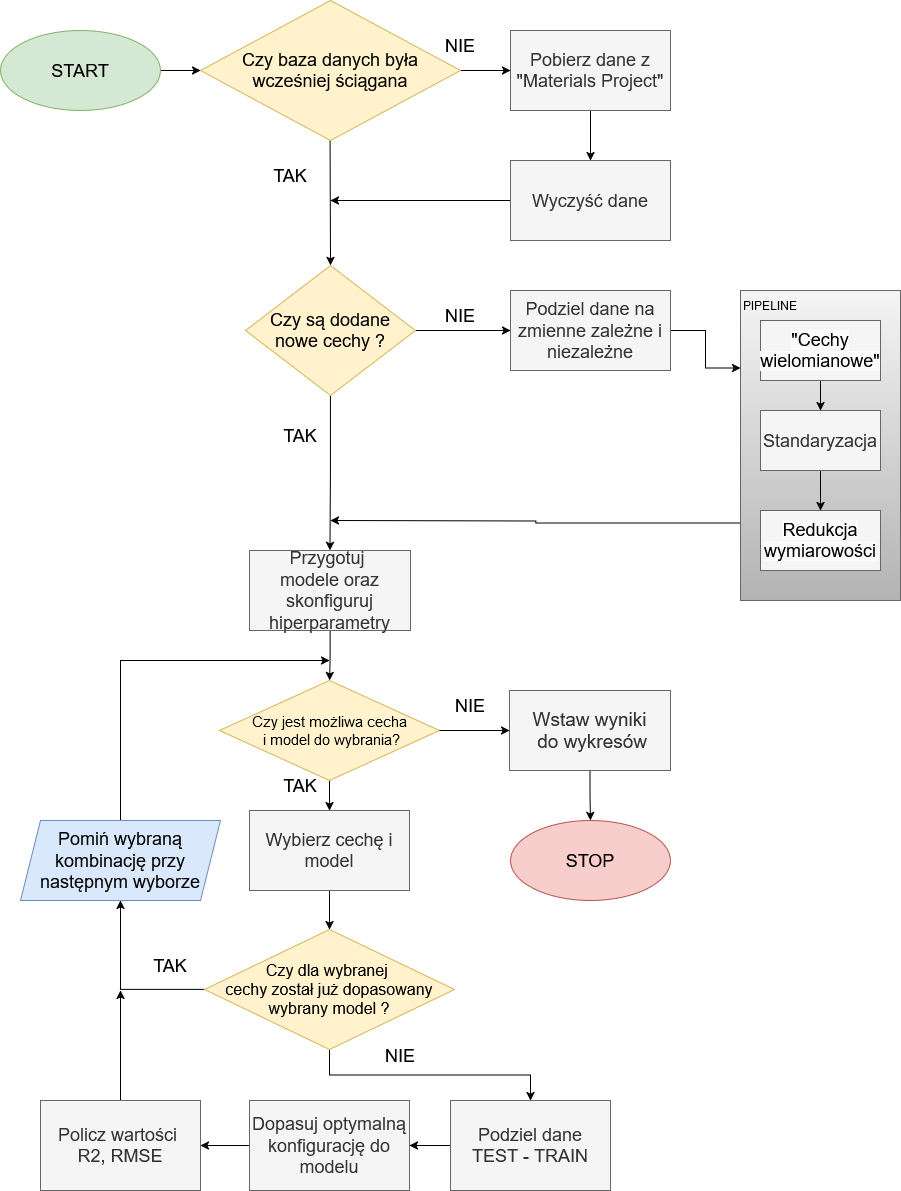
\includegraphics[width=\textwidth]{images/get df.drawio.png}
Schemat Blokowy opisujący proces działania programu.

\clearpage
